\documentclass[10.5pt]{article}
\usepackage[a4paper,margin=2.1cm]{geometry}
\usepackage{amsmath,amssymb}
\usepackage{booktabs}
\usepackage{graphicx}
\usepackage[hidelinks]{hyperref}
\usepackage{enumitem}
\usepackage{caption}
\usepackage{float}
\setlist{itemsep=1pt,topsep=2pt}
\captionsetup{font=small,labelfont=bf}
\newcommand{\code}[1]{\texttt{#1}}
\emergencystretch=3em
\author{Phung Gia Huy}
\date{November 2026}

\hypersetup{pdftitle={GStar Assignment 2, Problem 1: GRPO on Countdown},pdfauthor={Phung Gia Huy}}
\title{\textbf{GStar Assignment 2 -- Problem 1}\\[2pt]\large GRPO and Dr.GRPO on Countdown with Qwen3-1.7B}

\begin{document}
\maketitle
\vspace{-10pt}
\begin{center}\small
Code in this submission: \code{starter.py} (Tasks 1--5), \code{kaggle/} (training runner and notebook), \code{tests/}.\\
Analysis scripts (\code{report/}): \url{https://github.com/huypg-zenai/GStar-Assignment-2-GRPO}
\end{center}

\paragraph{Summary.}
\begin{itemize}
\item All four RL runs beat the 37\% target (the course's zero-shot accuracy at $L_{1024}$): GRPO 58.5\% / 52.1\% and
  Dr.GRPO \textbf{60.7\%} / \textbf{55.9\%} at $L_{256}$ / $L_{512}$, after 80 steps.
\item RL exploited the reward: 13--17\% of ``correct'' $L_{256}$ answers leave numbers unused, which the verifier (as
  specified) allows. Under the task's real rule the runs still score 48--55\%.
\item GRPO tends to commit to wrong answers and Dr.GRPO to run out of tokens. We attribute this to GRPO's std
  normalisation amplifying the 0.1 partial credit.
\end{itemize}

\section{Approach}
\textbf{Pipeline.} Each GRPO step samples 16 training prompts, syncs the policy into vLLM, generates a group of 8
responses per prompt, scores them with the reward function, and computes group-normalised advantages. It then runs the
PPO-style clipped loss over 32 gradient-accumulation micro-batches and takes one optimiser step.

\textbf{Implementation (Tasks 1--5, \code{starter.py}).}
\begin{itemize}
\item \code{compute\_group\_normalized\_advantages}: reshape rewards to \code{[prompts, G]}, subtract the group mean, and for
  GRPO divide by $\mathrm{std}+\epsilon$ (Dr.GRPO skips the division). Returns advantages, raw rewards and
  mean/std/max/min.
\item \code{compute\_loss}: per-token $-\min(A\rho_t,\;A\,\mathrm{clip}(\rho_t,1-\epsilon,1+\epsilon))$ with
  $\rho_t=\exp(\log\pi_\theta-\log\pi_{\theta_\text{old}})$; the advantage is broadcast over the response tokens.
\item \code{masked\_mean} (GRPO): mean over each response's tokens, then over the batch. \code{masked\_mean\_drgrpo}
  (Dr.GRPO): masked sum per response divided by a constant \code{num\_tokens} (the generation limit), then batch mean.
\end{itemize}
\code{tests/test\_tasks.py} checks every example from the handout plus edge cases (all pass).

\textbf{Compute setup.} We trained on Kaggle's free 2$\times$T4 GPUs instead of an A100, which forced three changes:
\begin{itemize}
\item \textbf{fp16} training with a gradient scaler, because T4s have no bf16;
\item \textbf{LoRA} adapters ($r=\alpha=32$, all linear layers) instead of full fine-tuning, to fit on one 16\,GB GPU;
\item \textbf{vLLM on the second GPU}, receiving the merged weights after every optimiser step.
\end{itemize}
\textbf{Hyper-parameters}, identical for all runs: 80 steps; 128 rollouts per step (16 prompts $\times$ 8); AdamW with lr
$5\times10^{-5}$; clip $\epsilon=0.2$; gradient-norm clip 1.0; temperature 1.0. Each $L_{256}$ run took about 1.7\,h and
each $L_{512}$ run about 3.2\,h.

\section{Reward design}
\begin{itemize}
\item \textbf{Verifiers (Task 1).} \code{\_extract\_answer} takes the \emph{last} \code{<answer>...</answer>}.
  \code{\_validate\_numbers} checks that the numbers used form a sub-multiset of those given (each used at most once), as
  the handout specifies. \code{\_evaluate\_equation} allows only digits, spaces and \code{+ - * / ( )}, rejects
  \code{**} and \code{//}, and returns \code{None} on any error (implicit multiplication, division by zero, Unicode
  operators).
\item \textbf{Reward (Task 2).}
  \begin{itemize}
  \item 1.0 if the equation is valid, uses allowed numbers, and evaluates to the target (tolerance $10^{-5}$);
  \item 0.1 if an \code{<answer>} tag is present but the answer is wrong for any reason;
  \item 0 if there is no tag.
  \end{itemize}
\item \textbf{Why the partial credit.} Zero-shot Qwen3 almost never finishes within 256 tokens, so a pure 0/1 reward
  would give no learning signal at the start. The 0.1 reward teaches the format first.
\item \textbf{Side effects.} The results below show two side effects of this design: answers that skip numbers count as
  correct, and the partial credit rewards guessing late in training.
\end{itemize}

\section{Evaluation methods}
\begin{itemize}
\item \textbf{Test set:} the 1,024 Countdown test prompts, with the course's prompt, sampling (temperature 1.0) and scoring
  from \code{zero\_shot\_eval.py}.
\item \textbf{Zero-shot:} at $L_{256}$, $L_{512}$ and $L_{1024}$.
\item \textbf{During training:} every 10 steps, plus the final model at step 80.
\item \textbf{Metrics:}
  \begin{itemize}
  \item accuracy (reward 1.0);
  \item correct / partial (0.1) / failed (0) counts;
  \item mean reward and output length.
  \end{itemize}
\item \textbf{Strict accuracy:} also requires every given number to be used exactly once, as the task statement says.
\item \textbf{Failure breakdown:} each response is put in one category using the reward's own verifier functions
  (\code{report/analyze\_p1.py}):
  \begin{itemize}
  \item correct;
  \item wrong value;
  \item invalid numbers or expression;
  \item no tag, cut off at the token limit;
  \item no tag, stopped on its own.
  \end{itemize}
\item \textbf{Training health:} on every step we compare vLLM's log-probabilities of the sampled tokens with the policy's.
  The gap stayed at 0.001--0.005 nats/token in all runs, so rollouts come from the current policy.
\end{itemize}

\section{Results}
\begin{table}[H]
\centering\small
\resizebox{\linewidth}{!}{%
\begin{tabular}{llccccc}
\toprule
Model & Max tokens & Accuracy & Strict acc. & Correct / partial / failed & Avg tokens & Best eval (step)\\
\midrule
Zero-shot & $L_{256}$ & 0.0\% & 0.0\% & 0 / 0 / 1024 & 256 & --\\
Zero-shot & $L_{512}$ & 9.0\% & 9.0\% & 92 / 21 / 911 & 498 & --\\
Zero-shot & $L_{1024}$ & 8.7\% & 8.7\% & 89 / 60 / 875 & 888 & --\\
\midrule
GRPO & $L_{256}$ & 58.5\% & 48.4\% & 599 / 310 / 115 & 139 & 58.5\% (80)\\
Dr.GRPO & $L_{256}$ & \textbf{60.7\%} & \textbf{52.9\%} & 622 / 36 / 366 & 161 & 61.1\% (70)\\
GRPO & $L_{512}$ & 52.1\% & 51.9\% & 533 / 10 / 481 & 374 & 52.1\% (70)\\
Dr.GRPO & $L_{512}$ & \textbf{55.9\%} & \textbf{55.3\%} & 572 / 10 / 442 & 356 & 55.9\% (80)\\
\bottomrule
\end{tabular}}
\caption{Accuracy on the 1,024 test prompts after 80 steps.}
\label{tab:p1}
\end{table}

\begin{figure}[H]
\centering
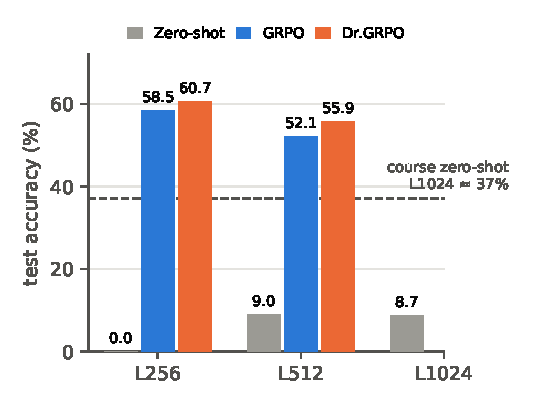
\includegraphics[width=0.49\linewidth]{figures/p1_accuracy.pdf}\hfill
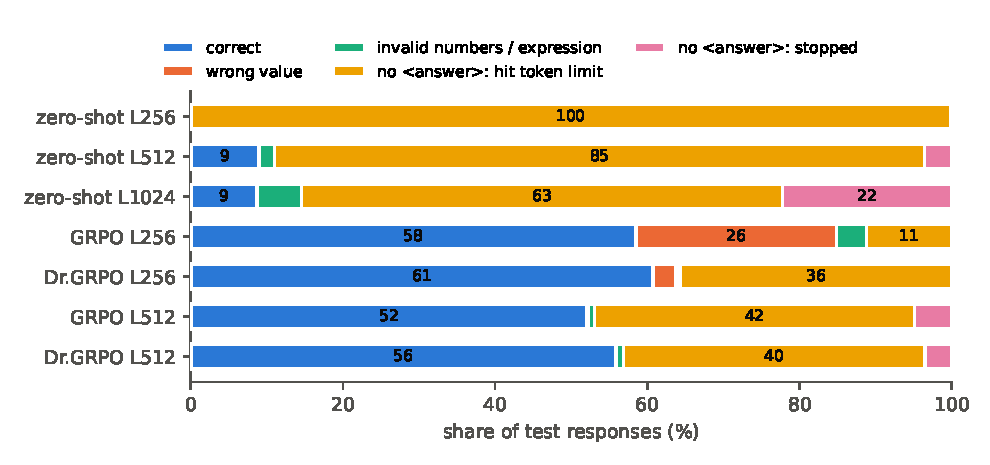
\includegraphics[width=0.49\linewidth]{figures/p1_failures.pdf}
\caption{Left: final accuracy vs zero-shot; the dashed line is the course's zero-shot $L_{1024}$ reference. Right: how
every test response ends.}
\label{fig:failures}
\end{figure}

\begin{figure}[H]
\centering
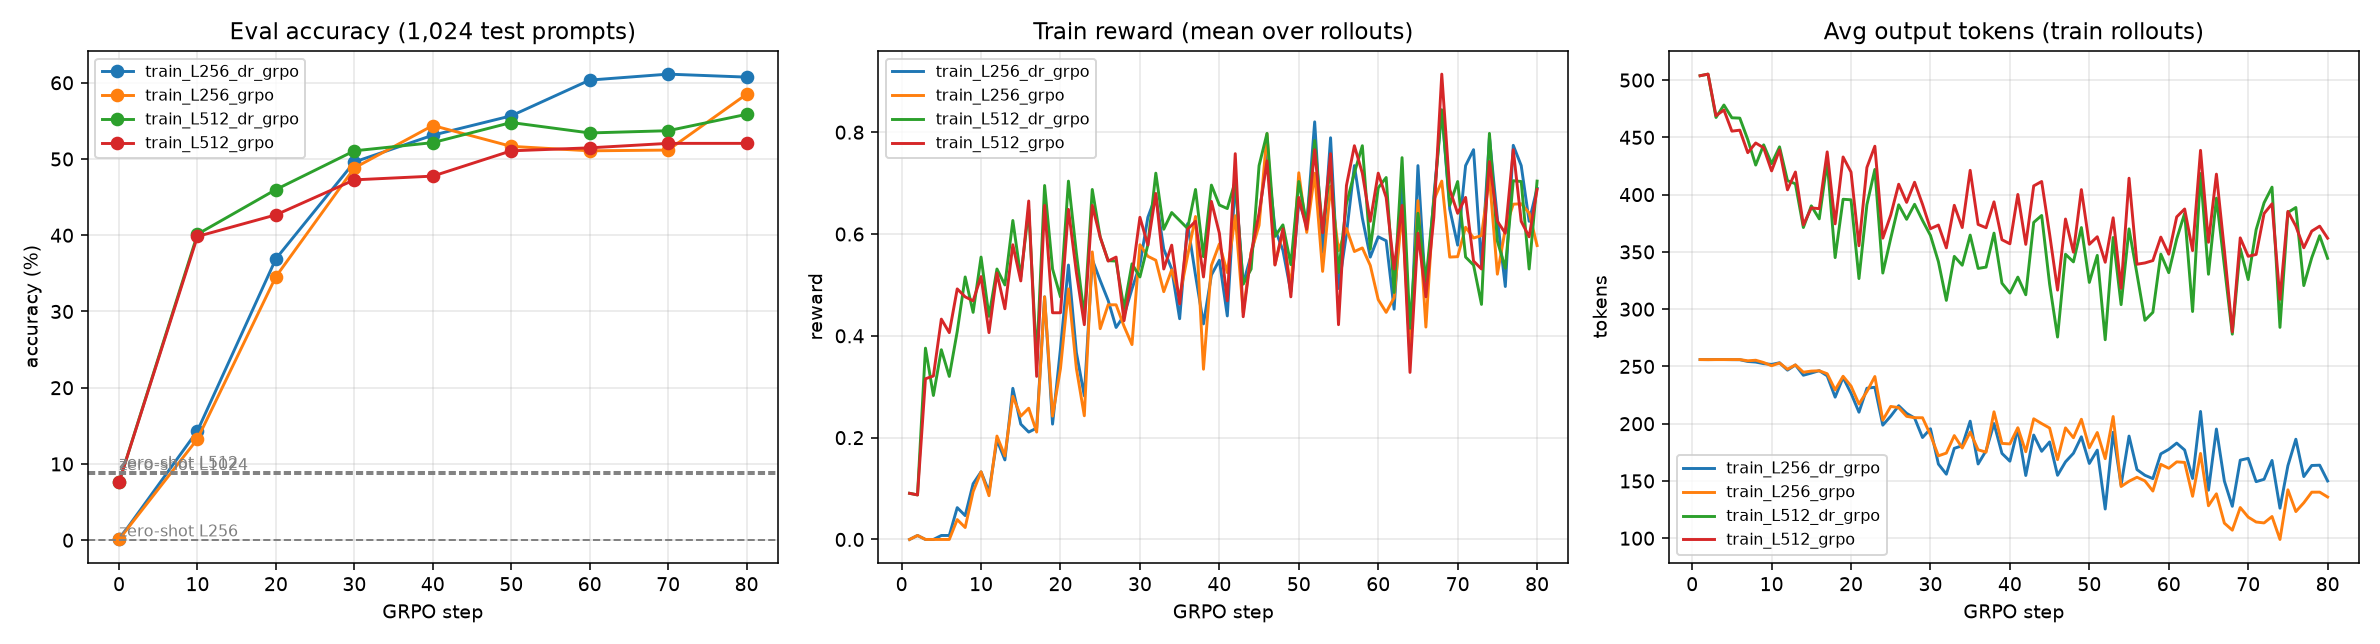
\includegraphics[width=\linewidth]{figures/p1_curves.png}
\caption{Training: test accuracy every 10 steps, mean training reward, and output length. No run became unstable within 80 steps.}
\label{fig:curves}
\end{figure}

\paragraph{Zero-shot is below the handout's numbers.}
\begin{itemize}
\item \textbf{The gap:} we get 0.0 / 9.0 / 8.7\% against the handout's 0.1 / 15 / 37\%. Prompt, sampling and scoring
  match \code{zero\_shot\_eval.py}, and the model weights are unchanged since release.
\item \textbf{The direct cause:} at $L_{1024}$, 63\% of answers hit the limit (often in loops such as ``45. 45. 45.'') and
  22\% stop without a tag. That caps accuracy at 37\%.
\item \textbf{Suspected reason:} fp16, forced by the T4s, may make long samples loop more often. We could not test bf16.
\item \textbf{Effect on the comparison:} none. Every run, baseline included, uses the same precision.
\end{itemize}

\section{Analysis}
\paragraph{Successful cases.}
\begin{itemize}
\item \textbf{Most of the gain is learning to finish.} Zero-shot answers are cut off 100\% of the time at $L_{256}$ and
  85\% at $L_{512}$. RL shortens $L_{256}$ answers from 256 to 139--161 tokens, into quick trial-and-error searches:
  ``79 $-$ 60 = 19, 17 + 19 = 36! \code{<answer>17 + (79 - 60)</answer>}''.
\item \textbf{Easy instances are solved.} Accuracy on 3-number problems is 79--84\% in every run, against 27--40\% on
  4-number problems. The 4-number problems need nested expressions that the greedy search rarely finds.
\item \textbf{Dr.GRPO beats GRPO at both lengths} (+2.2 and +3.8 points), and it is still improving at step 80 at $L_{512}$.
\end{itemize}

\paragraph{Failed cases.}
\begin{itemize}
\item \textbf{Reward hacking.}
  \begin{itemize}
  \item RL found that the verifier accepts any \emph{subset} of the numbers. 17\% (GRPO) and 13\% (Dr.GRPO) of correct
    $L_{256}$ answers skip numbers, for example \code{55 + 38} for target 93 with [55, 38, 69, 68].
  \item Zero-shot never does this, and the $L_{512}$ runs rarely do: tight budgets push the model to the cheapest
    equation that hits the target.
  \item Under the strict rule, $L_{512}$ beats $L_{256}$ for both methods.
  \end{itemize}
\item \textbf{GRPO guesses; Dr.GRPO runs out of tokens} (at $L_{256}$).
  \begin{itemize}
  \item GRPO gives a wrong value 26\% of the time against Dr.GRPO's 3\%; Dr.GRPO is cut off 36\% of the time against
    GRPO's 11\%.
  \item GRPO also learned an empty \code{<think></think>} and does its search outside it.
  \item \emph{Hypothesis:} in groups with no correct answer, the rewards are 0 (cut off) or 0.1 (any answer). GRPO divides
    by their small std, so ``write some answer'' earns advantages near $\pm1$, as large as for solving the problem.
    Dr.GRPO keeps that signal at $\le0.1$.
  \end{itemize}
\item \textbf{$L_{512}$ still truncates 40--42\%,} but almost never gives a wrong value (0--2 answers). Its problem is
  finishing, not accuracy.
\end{itemize}

\paragraph{What could be improved.}
\begin{enumerate}
\item Require every number exactly once in \code{\_validate\_numbers}.
\item Drop the 0.1 partial credit once the format is learned, or give it only to answers that use all numbers.
\item Skip groups with identical rewards: 38--68\% of groups late in training carry no gradient.
\item Use a soft length penalty or an $L_{256}\to L_{512}$ curriculum instead of hard truncation.
\item Retest the zero-shot gap on bf16 hardware.
\end{enumerate}

\section{Conceptual questions}
\paragraph{Clipping: more critical on- or off-policy?} Off-policy.
\begin{itemize}
\item The clip acts only when $\rho_t=\pi_\theta/\pi_{\theta_\text{old}}$ leaves $[1-\epsilon,1+\epsilon]$.
\item On-policy, the rollouts come from the parameters being updated, so $\rho_t=1$ and the loss is the plain policy
  gradient. That is our case: \code{old\_log\_probs = policy\_log\_probs.detach()}, with one optimiser step per batch, so
  the clip never fires.
\item When data is reused after the policy changes (several epochs, stale or asynchronous rollouts), $\rho_t$ drifts. The
  clip then stops a few high-advantage tokens from pushing the policy far from where the data was collected.
\end{itemize}

\paragraph{On-policy vs off-policy for this task.}
\begin{itemize}
\item \textbf{On-policy, advantage 1 -- unbiased gradient:} no importance weights and no $\epsilon$ to tune.
\item \textbf{On-policy, advantage 2 -- up-to-date baseline:} the group baseline reflects current behaviour, which changes
  fast here (length falls by a third within 30 steps at $L_{256}$).
\item \textbf{Off-policy, advantage 1 -- sample efficiency:} generation costs 15--33\,s per step, and early on 86--89\% of
  $L_{256}$ groups carry no signal, so reusing the rare successes is valuable.
\item \textbf{Off-policy, advantage 2 -- parallelism:} the two GPUs can generate and train at the same time with slightly
  stale weights, instead of waiting for each other.
\end{itemize}

\paragraph{Per-token gradients under the two reductions.} We ran the handout's batch through our \code{compute\_loss} and
both reductions and called \code{backward()} (\code{report/grad\_reductions.py}; $\rho=1$, the same advantage $A$ for both
responses, $B=2$, \code{num\_tokens}$\,=6$):
\begin{center}\small
\begin{tabular}{lccc}
\toprule
Reduction & per short-response token & per long-response token & total weight, short / long\\
\midrule
\code{masked\_mean} & $-0.167A$ & $-0.083A$ & $-0.5A$ / $-0.5A$\\
\code{masked\_mean\_drgrpo} & $-0.083A$ & $-0.083A$ & $-0.25A$ / $-0.5A$\\
\bottomrule
\end{tabular}
\end{center}
\begin{itemize}
\item \textbf{Observation:} \code{masked\_mean} weights each \emph{response} equally, so the short response gets twice the
  per-token gradient. \code{masked\_mean\_drgrpo} weights each \emph{token} equally, so a response's total weight grows with
  its length.
\item \textbf{Length bias:} with $A<0$, \code{masked\_mean} penalises long wrong answers less per token, which lets wrong
  answers grow longer.
\item \textbf{Prefer \code{masked\_mean}} when lengths vary widely and each sample should count equally, for example when
  a few very long truncated rollouts would otherwise dominate the update.
\item \textbf{Prefer \code{masked\_mean\_drgrpo}} for long chain-of-thought, where the length bias inflates wrong answers.
  Our $L_{512}$ runs fit this: Dr.GRPO answers are shorter (356 vs 374 tokens) and more accurate.
\end{itemize}
\end{document}
